\documentclass[9pt]{pnas-new}
% Use the lineno option to display guide line numbers if required.
% Note that the use of elements such as single-column equations
% may affect the guide line number alignment. 

%\RequirePackage[english,slovene]{babel} % when writing in slovene
\RequirePackage[slovene,english]{babel} % when writing in english
\usepackage{subcaption}

\usepackage[demo]{graphicx}
\templatetype{pnasresearcharticle} % Choose template 
% {pnasresearcharticle} = Template for a two-column research article
% {pnasmathematics} = Template for a one-column mathematics article
% {pnasinvited} = Template for a PNAS invited submission

%\selectlanguage{slovene}
%\etal{in sod.} % comment out when writing in english
%\renewcommand{\Authands}{ in } % comment out when writing in english
%\renewcommand{\Authand}{ in } % comment out when writing in english

\newcommand{\set}[1]{\ensuremath{\mathbf{#1}}}
\renewcommand{\vec}[1]{\ensuremath{\mathbf{#1}}}
\newcommand{\uvec}[1]{\ensuremath{\hat{\vec{#1}}}}
\newcommand{\const}[1]{{\ensuremath{\kappa_\mathrm{#1}}}} 

\newcommand{\num}[1]{#1}

\graphicspath{{./fig/}}

\title{Emotion contagion model for dynamical crowd path planning with panic}

% Use letters for affiliations, numbers to show equal authorship (if applicable) and to indicate the corresponding author
\author{Andrej Sušnik}
\author{Timotej Zgonik}
\author{Ema Leila Grošelj}

\affil{Collective behaviour course research seminar report} 

% Introduction, Methods, Results and Discussion

% Please give the surname of the lead author for the running footer
\leadauthor{Sušnik} 

\selectlanguage{english}

% Please add here a significance statement to explain the relevance of your work
% \significancestatement{Procedural generation of a tropic island and \\coral reef}{In computer graphics there is frequent need for displaying large vistas of natural looking terrain. Designing such terrain by hand is typically time consuming. With procedural generation, on the other hand, larger areas of natural looking terrain can be generated with or without minimal intervention in a relatively short time. In this work we present a process of procedural generation of a tropical island with the associated corral reef. We start by generating a heightmap for the base terrain. The heightmap is then transformed by simulating the processes of hydraulic and thermal erosion to achieve a more natural look of the terrain. As coral reefs often grow around tropical islands, we also simulate their growth as part of the last step. Real-time visualization is enabled during the simulation, so that one can observe the evolution of the terrain. Here we dynamically apply textures to the terrain based on its local characteristics. The result is a natural looking model of the textured tropical island and corral reef.}{Procedural generation | Terrain generation | Thermal and hydraulic erosion | Coral reef | Simulation | GPU}

%\selectlanguage{slovene}

% Please include corresponding author, author contribution and author declaration information
%\authorcontributions{Please provide details of author contributions here.}
%\authordeclaration{Please declare any conflict of interest here.}
%\equalauthors{\textsuperscript{1}A.O.(Author One) and A.T. (Author Two) contributed equally to this work (remove if not applicable).}
%\correspondingauthor{\textsuperscript{2}To whom correspondence should be addressed. E-mail: author.two\@email.com}

% Keywords are not mandatory, but authors are strongly encouraged to provide them. If provided, please include two to five keywords, separated by the pipe symbol, e.g:
\keywords{Dynamic crowd path planning | Crowd behavior | Simulation | Emotion contagion} 

\begin{abstract}
% An emotion contagion model for dynamical crowd path planning would allow for realistic and plausible simulation of crowd path planning and crowd behavior. Modeling agents' personalities using the OCEAN, or big five, personality trait model allows us to simulate a diverse crowd that reacts to the environment in different ways, while also affecting neighboring agents and their path planning. As an addition to the original model, we tried to implement a panic parameter to add an element of randomness to the agents' movements.
%%%%%%%%%%%%%%%%%%%%%%%%%%%%%%%%%555
% V okviru tega članka smo implementirali An emotion contagion model for dynamical crowd path planning iz članka \cite{Wu_Huang_Tian_Yan_Yu_2024}. Gre za model, ki poskuša modelirati obnašanje množice ljudi med evakuacijo v primeru požara. Njihove osebnosti so predstaveljne z OCEAN modelom. Simulate a diverse crowd that reacts to the environment in different ways. Karakteristike se spreminjajo glede ljudi in nevqrnosti v okolici. V ospredju je modeliranje dileme med tem, ali naj izberejo najbližji izhod, ali pa morda raje poskusijo svojo srečo pri bolj oddaljenem, a manj zasedenem izhodu. 

% To kateri ljudje so v naši okoljici, določimo gručenjem. Algoritem za gručenje iz \cite{Wu_Huang_Tian_Yan_Yu_2024} smoprimerjali z drugimi algoritmi. Dodali smo koncept panike. Bolj panični agenti se bolj panično, nepredvidljivo gibljejo po prostoru. Agente smo pravtako postavili pred različne ovire, na primer v pisarni.
%%%%%%%%%%%%%%%%%%%%%%%%%%%%%%%%5
In this article, we implement An Emotion Contagion Model (ECM) for Dynamical Crowd Path Planning from \cite{Wu_Huang_Tian_Yan_Yu_2024}. This model aims to simulate crowd behavior during fire evacuations, considering individuals’ personalities based on the OCEAN personality model. The simulation captures a diverse crowd that reacts to the environment in different ways, with agent characteristics evolving based on surrounding individuals and fire sources.

A key focus of the model is the dilemma individuals face when choosing between the nearest exit or opting for a farther but less congested route. Surrounding individuals are estimated by employing clustering techniques. The clustering algorithm by Wu et al. [2024] is compared against other clustering methods. Additionally, we introduce the concept of panic — agents experiencing higher panic levels exhibit more erratic and unpredictable movement patterns. The simulation also incorporates obstacles, such as an office environment, to test agent behavior under constrained conditions.

\end{abstract} 

\dates{\textbf{\today}}
\program{BM-RI}
\vol{2024/25}
\no{CB:GB} % group ID
%\fraca{FRIteza/201516.130}

\begin{document}

% Optional adjustment to line up main text (after abstract) of first page with line numbers, when using both lineno and twocolumn options.
% You should only change this length when you've finalised the article contents.
\verticaladjustment{-2pt}

\maketitle
\thispagestyle{firststyle}
\ifthenelse{\boolean{shortarticle}}{\ifthenelse{\boolean{singlecolumn}}{\abscontentformatted}{\abscontent}}{}

% If your first paragraph (i.e. with the \dropcap) contains a list environment (quote, quotation, theorem, definition, enumerate, itemize...), the line after the list may have some extra indentation. If this is the case, add \parshape=0 to the end of the list environment.

% INTRO
\section{Introduction}
% \dropcap{I}ntroduction: 
Efficient crowd path planning is crucial in various real-world applications, from urban transportation management to emergency evacuations. Wu et al. [2024] present an innovative approach by integrating emotional dynamics into crowd behavior modeling, offering a look into how individual emotions influence collective movement patterns. Their model is called an Emotion Contagion Model (ECM).

This project aims to reproduce the results of the original study to validate its findings and explore potential improvements and other adjustments.

% METHODS
% \dropcap{M}ethods: 
\section{Methods}
\subsection{Related work} 

The key components of the emotion contagion model are shown in \ref{fig:outline}, and are further explained below. 
\begin{figure}[h!]
    \centering
    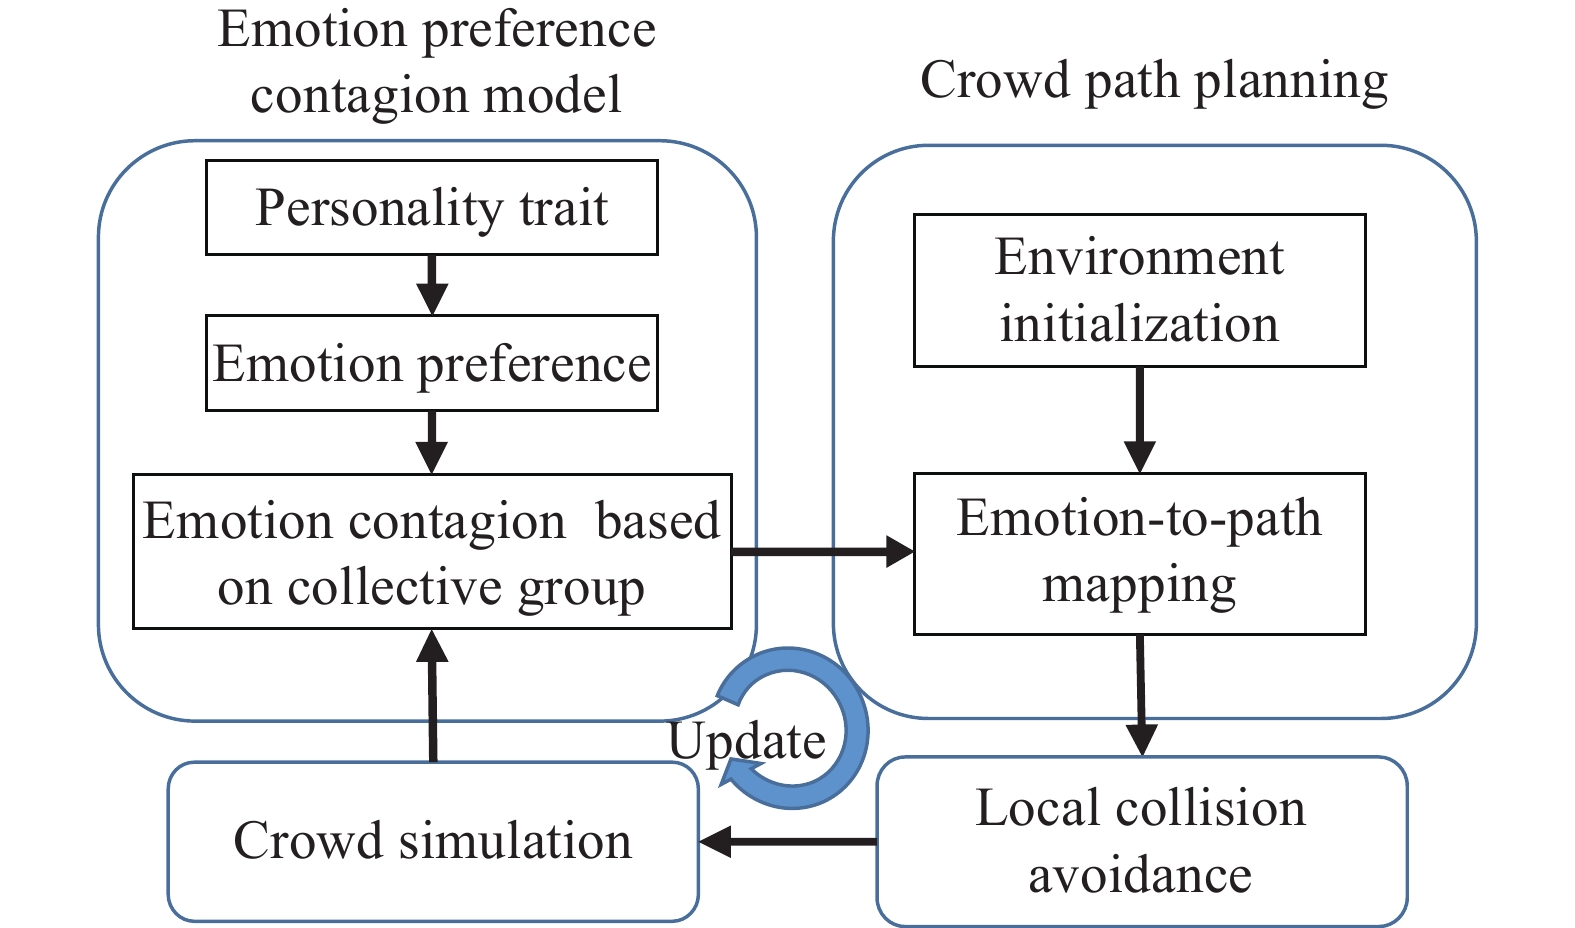
\includegraphics[width=0.6\linewidth]{fig/outline.jpg}
    \caption{The emotion contagion model as proposed by Wu et al. [2024].}
    \label{fig:outline}
\end{figure}

\subsubsection{Trait model and mapping to the least time consuming exit}
The source article proposes generating agents with distinct values for the five OCEAN traits: openness to experience, conscientiousness, extroversion, agreeableness, and neuroticism. Based on those factors, agents are then assigned an initial distance preference ${P_d}$ and an initial velocity preference ${P_v}$. Agents have larger distance preferences if their personality factors are simple, aggressive, and fragile (corresponding to OCEAN factors: O${-}$, E${-}$, A${+}$), and agents have larger velocity preferences if their personality factors are variable, energetic, and functional (corresponding to OCEAN factors: C${-}$, E${+}$, N${+}$). If an agent has a large distance preference, its velocity preference is usually smaller, and vice versa. An agent with a larger velocity preference will seek to find less crowded paths even at the cost of the distance being longer, while those with a larger distance preference will stick to a path even as it becomes crowded. The model incorporates a strategy where a least expected-time objective function is used to dynamically select paths, factoring in both environmental variables and agents’ emotional states and preferences \cite{Wu_Huang_Tian_Yan_Yu_2024}.

\subsubsection{Change of traits by emotion contagion and other sources}
An emotion contagion mechanism further enhances the model by allowing emotional states to spread among neighboring agents, mimicking the way emotions such as stress or calm influence a group. A dampening factor regulates this contagion to ensure an agent's inherent personality traits are at least partially preserved. For contagion of emotions, the simulation requires a method to define collective clusters among the agents to determine which of them will be mutually affected. Agents are defined as being collective neighbors if they share similar motion or have a mutual goal. Information is contagious between neighboring agents in the same group and is affected by the distance between agents and the difference between emotion preferences. Wu et al. [2024] propose an algorithm that begins by identifying the agent with the highest density as the centre of the first cluster. It then evaluates each remaining agent in order of increasing density, checking whether it belongs to an existing cluster based on its distance to the nearest high-density agent. If no cluster matches, a new one is created. Additionally, agents may be affected by environmental contagious sources, such as a fire disaster \cite{Wu_Huang_Tian_Yan_Yu_2024}.  

\subsubsection{Panic contagion and influence}
Wang et al. [2022] describe how panic could influence the path planning of an agent.
The authors propose a model where panic is contagious and negatively impacts the ability of an agent to find an exit.

\subsection{Proposed additions}
% Emotion memory
% We propose adding an additional \textbf{Emotion memory} parameter to the agents. The emotion memory parameter would affect the agent on a multi-run simulation where the same agents would be placed in different environments in sequence.

\subsubsection{Panic}
To introduce the concept of \emph{panic} to the simulation, each agent is assigned a \emph{panic parameter} and a \emph{panic susceptibility parameter}, where panic inhibits the ability of the agent to move to their goal. As the panic parameter increases, the agent's movement becomes increasingly erratic and random.

\emph{The panic susceptibility parameter} - how susceptible is someone to surrounding panic, in our approach, is calculated from the OCEAN traits of the agent, as shown in Equation \ref{equ:panic}. The subscript $_0$ next to a given trait denotes the value being shifted by $0.5$ from the original expected value, so that the new expected value is equal to $0$. Openness, conscientiousness and agreeableness have negative correlation with panic susceptibility, while neuroticism has positive correlation. The distribution of panic susceptibility remains equal to the distribution of the traits: $N(0.5,0.1)$. We decided that all traits are equally important: \(w_O = w_C= w_A= w_N= \sqrt{1/4}\).

\begin{align}
    \label{equ:panic}
    panic\_susceptibility = -w_O * O_0 - w_C* C_0 - w_A* A_0 + w_N *  
    N_0 + 0.5, \\
    \text{where } w_O^2 + w_C^2 + w_A^2 + w_N^2 = 1 \nonumber
\end{align}

Each agent is also assigned a current \emph{panic parameter}. This parameter represents the probability that the agent will not behave according to their personality and will either freeze or move randomly. This parameter can be modified in three ways. Every agent seeks to reduce their panic to a baseline level, the return to the baseline level being dependent on their panic susceptibility parameter. The relationship is described in Equation \ref{equ:panic_decress} for every $\Delta{t}$.

\begin{equation}
    current\_panic \mathrel{-}= (0.5 + (0.01 - 0.5) \cdot panic\_susceptibility) * (current\_panic)
    \label{equ:panic_decress}
\end{equation}

There are two means by which the panic parameter of an agent may increase. Agents are susceptible to the panic of other agents in their cluster and their panic parameter value will accordingly change to match the cluster's average, with the speed of the change governed by their panic susceptibility, as described by Equation \ref{equ:panic_clustenr_inc}. 

\begin{equation}
  \begin{aligned}
    panic\_\text{\textit{diff}} = average\_cluster\_panic - current\_panic \\
    current\_panic \mathrel{+}= panic\_susceptibility * panic\_\text{\textit{diff}} * 0.05
\end{aligned}
    \label{equ:panic_clustenr_inc}
\end{equation}

An agent's current panic may also increase if they are near a panic-inducing source, which is described by Equation \ref{equ:panic_inuction}.
\begin{equation}
    \begin{aligned}
        dist = \frac{1} {|position - panic\_source\_position|} \\
        current\_panic += dist * panic\_susceptibility * 0.001
    \end{aligned}
    \label{equ:panic_inuction}
\end{equation}

\subsubsection{Clustering algorithm evaluation}
To implement the emotion contagion, we need to identify the community clusters. The clustering as proposed by Wu et al. [2024] operates as follows: two agents are neighbors if they have the same exit as a goal or if they at least have a similar position and direction. Moving from the agents with most neighbors to the ones without them, we merge clusters so that an agent is in the same cluster as its closest neighbor with a higher or equal degree.
Wu et al. [2024] do not provide any reasoning as to why a specialised clustering algorithm was necessary, so as part of this project, we chose to evaluate the performance of their clustering algorithm by comparing it to hierarchical clustering and Fast Label Propagation \cite{Lovre_2023}.
% generalized community detection algorithms, such as Leiden \cite{Leiden}, Walktrap \cite{Walktrap}, or (Fast) Label Propagation \cite{Lovre_2023}.

% We plan to test how the grid resolution affects the movement of agents.

\subsubsection{Enhanced navigation graph} When an agent chooses an exit, we need to also choose a path that leads from an agent's current position to their chosen exit. This is efficiently done with pre-computing a navigation graph that stores all the shortest paths to a given exit. Additional movement options have been added to the navigation graph, as described in Section \ref{res}.


\subsubsection{Corrected error}
We believe to have found \textbf{an error in the source article} with its equation: \begin{equation*}
    d_{ori}(i,j)=|arccos(vel_i)-arccos(vel_j)|
\end{equation*}
which does not appear to be a operation that can be performed on a vector, so we instead propose: \begin{equation*}
    d_{ori}(i,j)=|atan2(vel_{i_y},vel_{i_x})-atan2(vel_{j_y},vel_{j_x})|
\end{equation*}
where we obtain the correct angle ${\theta}$\ from the \textit{x}-axis \cite{wikiatan2} for each of a pair of agents and then subtract the angles to obtain the difference between their orientations. The article does not acknowledge why this was used instead of a dot product, and in good faith, we assumed there must have been a reason for that decision.

% RESULTS
\section{Results} \label{res}
%\subsubsection{Clustering}
%Figure \ref{fig:enter-label} shows multiple runs of the clustering algorithm from article \cite{Wu_Huang_Tian_Yan_Yu_2024}. Even though %the clusters were very different when we used a different algorithm, little to no effect was visible on the agent paths.

%\begin{figure}[h!]
%    \centering
%    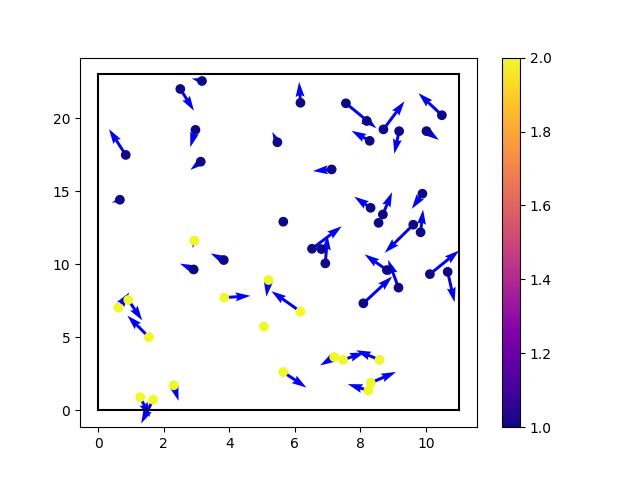
\includegraphics[width=0.3\linewidth]{fig/Figure_2.png}
%    \hfill
%    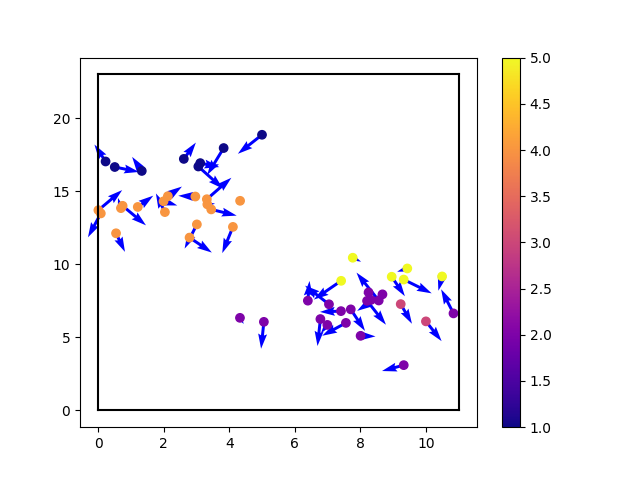
\includegraphics[width=0.3\linewidth]{fig/Figure_3.png}
%   \hfill
%   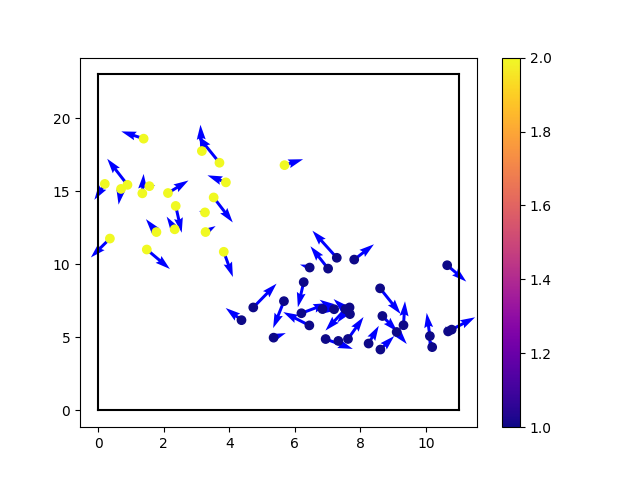
\includegraphics[width=0.3\linewidth]{fig/Figure_4.png}
%   \caption{Example runs of clustering according to association with the closest neighbor with a higher degree. The leftmost sub-figure represents agents with positions initialized uniformly, while the two to the right represent agents with positions initialized with a bimodal Gaussian distribution.
%   Every distinct colour represents a different cluster of agents, that is, the middle sub-figure has five clusters, while the others have only two. }
%    \label{fig:enter-label}
%\end{figure}

\subsubsection{Navigation graph}

For each exit, we constructed a navigation graph of shortest paths. Every such graph is a tree or a forest with roots among the nodes belonging to an exit, representing the shortest paths from all possible positions on the grid to one of the exits. It was constructed using Dijkstra's algorithm, allowing movements to all 8 neighboring fields as well 
as to fields located two steps in one direction and one step in a perpendicular direction.
An example graph is shown in Figure \ref{fig:spgraph}.

This navigation graph would, in theory, allow for modeling the movement of agents in a more natural way than the basic left-right-up-down version of it.

\begin{figure}[h!]
    \centering
    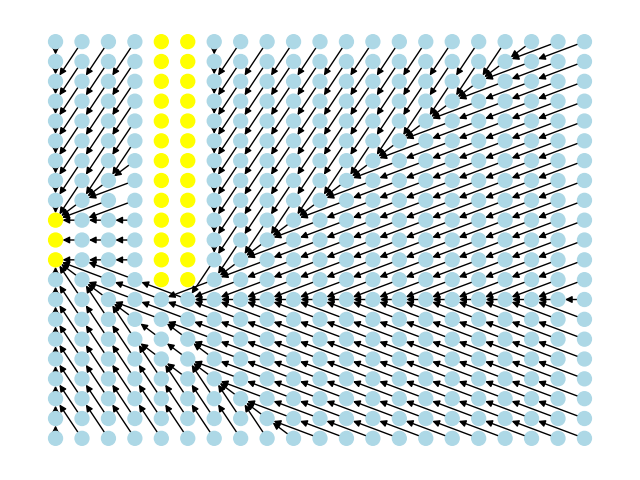
\includegraphics[width=0.5\linewidth]{fig/dijkstra.png}
    \caption{Example navigation graph for a grid of dimensions 10 times 10. Yellow nodes represent the exit of width 3 and the obstacle. Every blue node has its shortest path towards the exit nodes show.}
    \label{fig:spgraph}
\end{figure}

\subsubsection{Performance evaluation} To test the limits of our implementation, we conducted a performance evaluation. We used a 256 x 256 grid as an environment and ran the simulation on a machine with an Intel i5-1260P CPU and 16 GB of RAM. Table \ref{tbl:preformance} shows the results, showing that when the number of agents is smaller or equal to 200, the performance could be considered real-time (above 30 frames per second). When we increased the number of agents, the frame rate dropped significantly, reaching only a single frame per second with 1000 agents. Upon profiling the code, we determined that the major bottlenecks were cluster formation and the contagion of emotional preferences step. 
\begin{table}[h!]
\begin{tabular}{ll}
Num. agents & Average frames per second \\
10          & 290         \\
50          & 263         \\
100         & 172         \\
200         & 70          \\
500         & 10          \\
1000        & 1.5          
\end{tabular}
\caption{Results of performance evaluation}
\label{tbl:preformance}
\end{table}

\begin{figure}[h!]
    \centering
    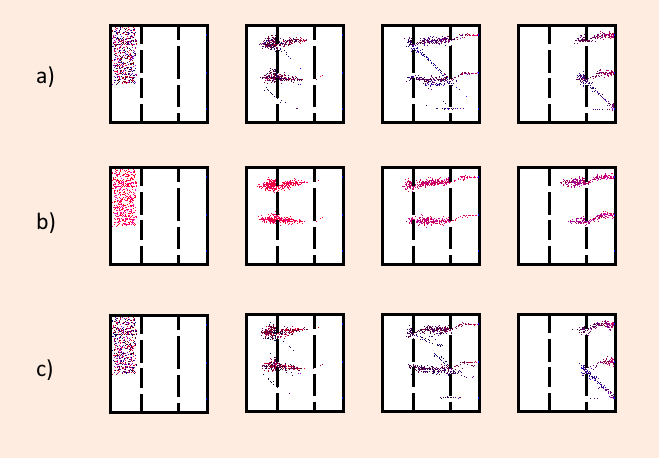
\includegraphics[width=\linewidth]{fig/clustering.png}
    \caption{The demonstration of crowd path planning with different emotion preferences and different clustering algorithms. In all cases, the screenshots are taken at frames 1, 25, 55 and 100 of the simulation. Blue dots indicate agents with a high velocity preference, while red dots indicate those with a high distance preference.}
    \label{fig:demo}
\end{figure}

\subsubsection{Crowd path planning under different emotion preferences}
Figure \ref{fig:demo} shows the results of the simulation under different initial parameters. 
In a), around 50\% of agents have a high distance preference and the other 50\% have a high velocity preference. Agents with a high velocity preference avoid congestion, opting for exits farther away. When agents are near an exit, emotion contagion takes effect, reducing the aggressiveness of all agents, including those with a preference for velocity.  
In b), all agents have a high distance preference. They are all willing to wait in lines and almost no agent chooses an exit that is farther away. 
In c), around 50\% of agents have a high distance preference and the other 50\% have a high velocity preference. We use hierarchical clustering instead of clustering algorithm proposed by Wu et al. [2024]. Hierarchical clustering creates smaller clusters, reducing the time it takes the agents to reach the destination. 

\subsubsection{Panic}
We discovered that the panic parameter has great influence on the paths, as shown in Figure \ref{fig:panic}. Without accounting for crowd panic, all the paths are very efficient, which is not necessarily the most accurate reflection of a real-world evacuation. When exposed to a contagious source such as fire, agents behave erratically the closer they are to the panic source.

\begin{figure}[h!]
    \centering
    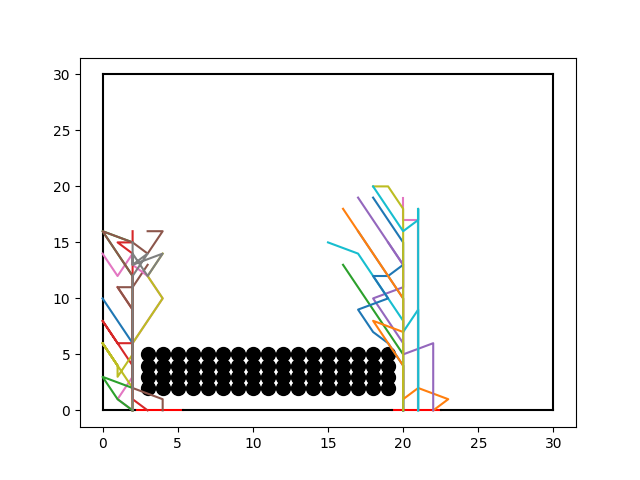
\includegraphics[width=0.45\linewidth]{fig/path_plot_nopanic.png}
    \hfill
    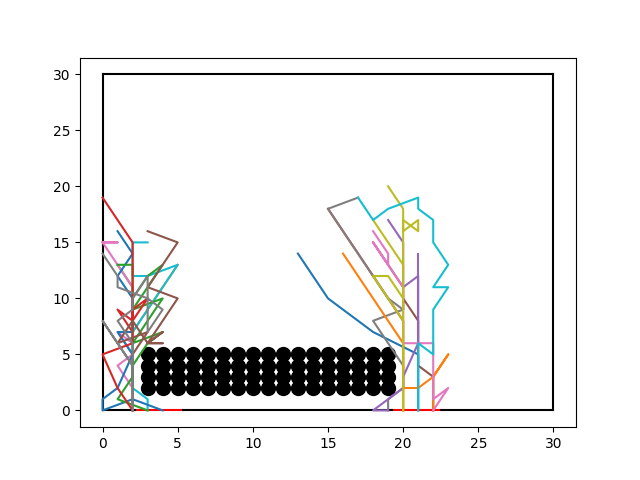
\includegraphics[width=0.45\linewidth]{fig/path_plot_panic.png}
    \caption{Example runs without a source of panic (left) and with a source of panic (right) included. The more erratic movement as a result of the panic is clearly seen in the right part of the figure.}
    \label{fig:panic}
\end{figure}

% DISCUSSION
\section{Discussion}
We have implemented a simulation workflow where we can define the environment with a bitmap image and then run the simulations. We compared the hierarchical clustering algorithm with the algorithm described in the source article and found that hierarchical clustering usually provides better results. The introduction of a panic parameter induced panic-like behavior into the paths of agents, bringing the simulation closer to real-life scenarios.

Many aspects of the implementation had to be reinvented, as Wu et al. [2024] at some points did not elaborate on their solutions. One such instance was with the implementation of the navigation graph generation, as for small environment sizes in the range of $100\times 100$ tiles were reasonably fast, but larger environments were not feasible as the time to construct the graph was excessive. To allow for greater precision of agent movement, it would be preferable to optimize the navigation graph generation or at least cache it for repeated use.

Future work could explore alternatives for the navigation graph that would allow for the agent positions to be points instead of real numbers. Additionally, the agent paths could be curves parametrized by continuous time parameters, which would allow for continuous time instead of discrete time steps. Another thing that could be explored in further work is the optimization of clustering algorithm and contagion of emotional preferences, so we could test larger number of agents.

\acknow{\textbf{AS} worked on the code (environment representation, agent movement, density calculation, code optimization) and on the report, \textbf{TZ} worked on the report and its editing as well as proofreading, and oversaw project management, and \textbf{ELG} worked on the code (contagion, navigation graph, clustering, visualization) and on the report.}
\showacknow % Display the acknowledgments section

% \pnasbreak splits and balances the columns before the references.
% If you see unexpected formatting errors, try commenting out this line
% as it can run into problems with floats and footnotes on the final page.
%\pnasbreak

\begin{multicols}{2}
\section*{\bibname}
% Bibliography
\bibliography{./bib/bibliography}
\end{multicols}

\end{document}